\chapter{Robots in agriculture}
\section{Robotics in Agriculture}
In 2025, agricultural robotics is at the forefront of transforming farming practices with cutting-edge technology. Key advancements include fully autonomous tractors, like John Deere's 2025 models, which perform tillage functions without human intervention, increasing efficiency and reducing labor costs [\cite{DeereCES2025}]. Precision harvesting robots, such as those from Harvest CROO, address labor shortages by picking crops like strawberries with precision and speed, reducing post-harvest losses. Drones play a crucial role in crop monitoring and precision spraying, enabling farmers to make data-driven decisions and optimize resource use [\cite{BuiltInAgRobots}]. Sophisticated weeding and planting robots, like Lettuce Bot from Blue River Technology (now part of John Deere), reduce herbicide use and manual labor by autonomously thinning and weeding fields [\cite{Robovision2025}]. 

\subsection{Robotic manipulators in agriculture}
The state-of-the-art in agricultural robotics encompasses a wide range of applications, each addressing specific challenges in farming. Below, we detail the major categories and examples:
Autonomous Tractors and Vehicles:
One of the most significant developments is the introduction of fully autonomous tractors. For instance, John Deere revealed new autonomous machines at CES 2025, with driverless autonomy systems available for model year 2025 and newer 8R and 9R tractors, initially for tillage functions [\cite{DeereCES2025}]. These tractors can operate without human intervention, reducing labor costs and increasing efficiency. This aligns with the trend of precision farming, where GPS and AI enable precise navigation and task execution. In general, application of robotics in agriculture can be divided into two sections:






\textbullet \,\textbf{ Precision Harvesting Robots}:
Harvesting robots are transforming labor-intensive tasks, particularly for delicate crops. Companies like Harvest CROO specialize in strawberry harvesting robots that can navigate uneven terrain and pick at human speed, addressing labor shortages and minimizing waste [\cite{BuiltInAgRobots}]. These robots are designed to handle soft crops, reducing post-harvest losses and improving yield efficiency. Another example is the Lettuce Bot from Blue River Technology (acquired by John Deere in 2017), which autonomously thins and weeds lettuce fields, reducing reliance on herbicides . Aotearoa New Zealand’s apple industry faces labor shortages for skilled tasks like thinning, prompting the development of an automated robot that scans both sides of tree canopies to accurately map fruitlets (81\% accuracy) and estimate size (5.9\% RMSE). The system addresses visibility challenges in dense foliage, proving more effective than single-sided scans (73.7\% accuracy) as shown the \ref{fig:applerobot} .

\begin{figure}
    \centering
    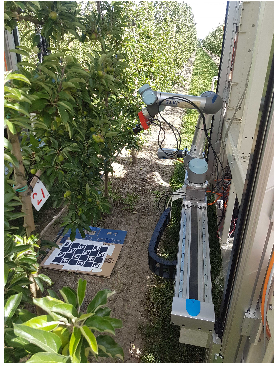
\includegraphics[width=0.5\linewidth]{pictures/robot_pickingapple.png}
    \caption{Internal view of one of the UR5 robotic arms mounted on the linear rail system used to scan the apple trees. [\cite{robotApple}]}
    \label{fig:applerobot}
\end{figure}

This research presents a cooperative grape-harvesting system using two heterogeneous robots—an 'expert' for picking and a 'helper' for transport—to address farm labor shortages and improve efficiency. Field experiments validated the navigation and collaboration strategy, while future enhancements explore logic-based decision-making for autonomous agricultural robots[\cite{robot_grape}].
\begin{figure}
    \centering
    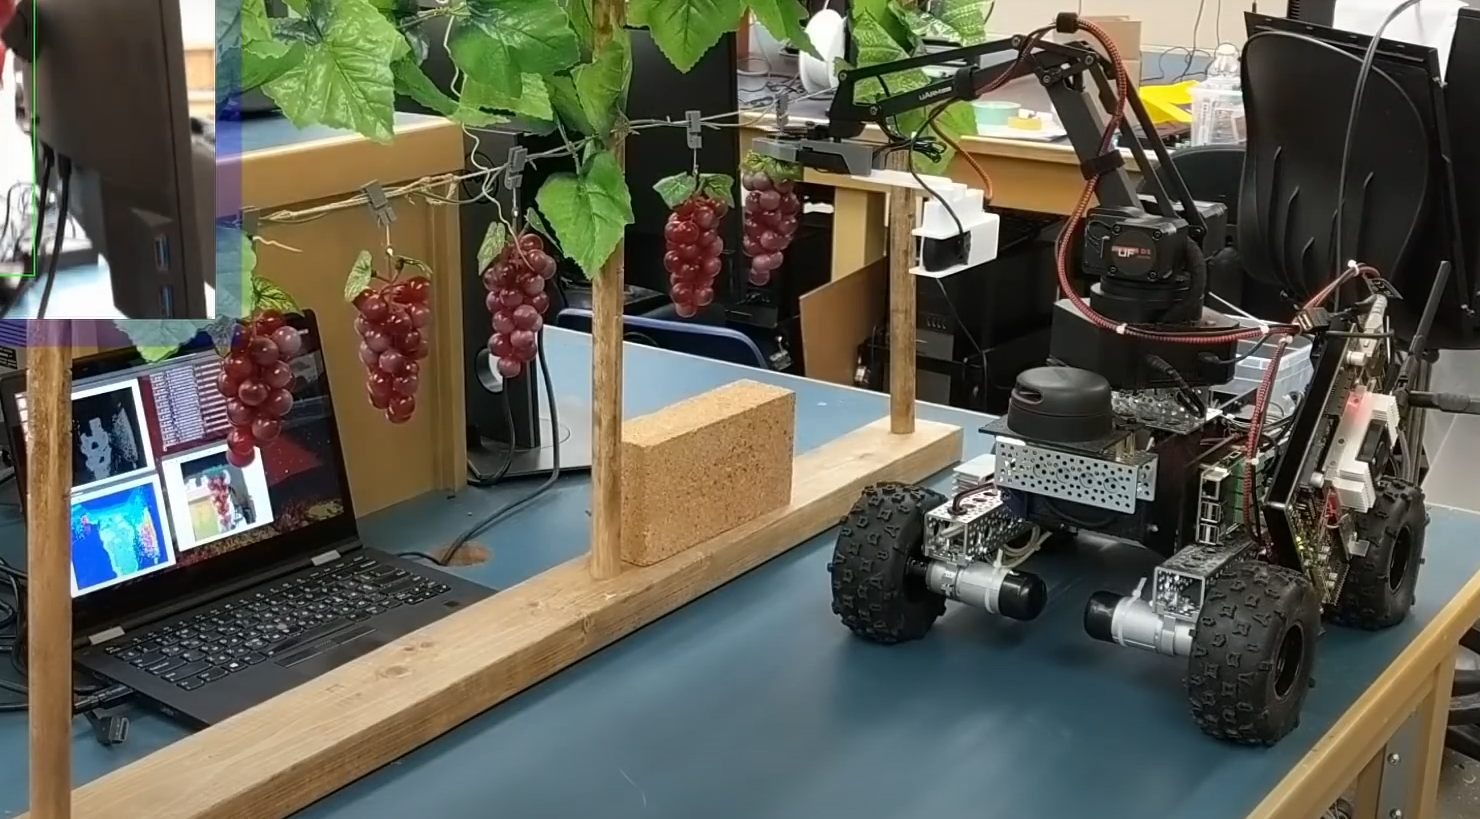
\includegraphics[width=0.75\linewidth]{pictures/grape_robot.png}
    \caption{experimental robot arm picking grapes in lab setup[\cite{robot_grape}]}
    \label{fig:enter-label}
\end{figure}


SWEEPER, the pioneering sweet pepper harvesting robot, achieves 61\% success in optimized greenhouse conditions with 24-second harvest cycles, proving robotics' potential while highlighting the need for crop adaptation. Its commercial-scale testing (262 fruits) reveals critical trade-offs between speed, accuracy, and real-world agricultural constraints[\cite{SweeperProject}].

\begin{figure}
    \centering
    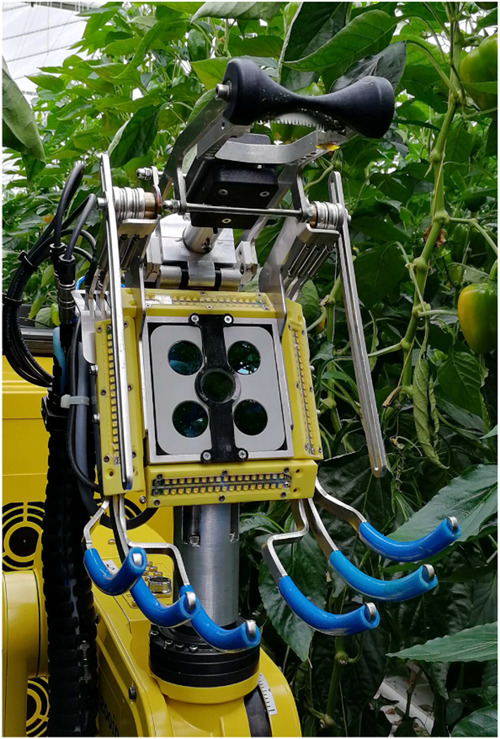
\includegraphics[width=0.5\linewidth]{pictures/bell_pepper.jpg}
    \caption{sweeper robot picking bell pepper}
    \label{fig:enter-label}
\end{figure}

\textbullet \,\textbf{ Weeding and Planting Robots}:
Robotic systems for weeding and planting are becoming more sophisticated, addressing the need for precision and reduced chemical use. The OMEGA robot from Terra Robotics, for example, uses laser technology for autonomous weeding, eliminating the need for chemical herbicides and promoting organic farming [\cite{TerraRobotics}]. Planting robots, often equipped with GPS, ensure optimal seed spacing and depth, improving crop uniformity and yield. These innovations are crucial for sustainable agriculture, reducing environmental impact and labor costs. Carbon Robotics develops AI-powered agricultural robots, specializing in autonomous weed control systems using laser technology to enable sustainable, precision farming. Their flagship product is the 'LaserWeeder' designed to reduce herbicide use while improving crop yields[\cite{CarbonRobotics}].

\subsection{Compliant Grippers in Agricultural Robotics}
The development of effective robotic end-effectors for horticulture remains a significant challenge due to the irregular shapes, fragile textures, and variable sizes of fruits and vegetables. While robotic grippers have been studied for decades, most existing designs are narrowly tailored to single crops like tomatoes or strawberries, limiting their versatility in real-world agricultural applications. Compliant materials emerge as a promising solution, enabling end-effectors to conform gently to produce surfaces, distribute pressure evenly, and minimize damage during handling. Traditional rigid fingers, though mechanically simple, lack adaptability, while articulated designs introduce control complexity without guaranteeing reliability. This study focuses on medium-sized spherical fruits (e.g., apples, tomatoes) with diameters of 40–100 mm, using ripe tomatoes—a worst-case scenario due to their low Young’s Modulus (2.32 MPa)—as a benchmark for gripper design[\cite{russo2017design}]


\begin{figure}
    \centering
    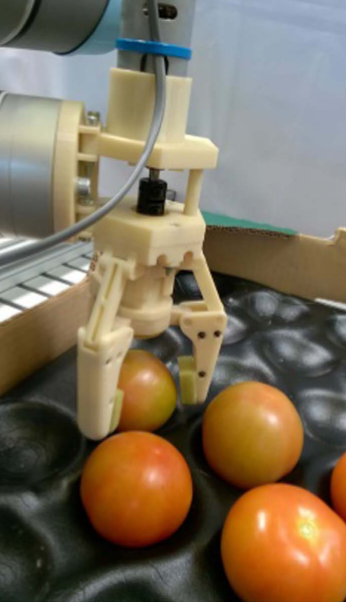
\includegraphics[width=0.5\linewidth]{pictures/tomato_gripper.png}
    \caption{testing a gripper design on different quality of tomatos [\cite{russo2017design}]}
    \label{fig:enter-label}
\end{figure}


this study introduces eight innovative 1-degree-of-freedom end-effectors based on deployable scissor mechanisms, which can compactly fold and expand to harvest single or multiple fruits while offering both direct-fruit and stem-holding separation methods. Validated through 3D-printed prototypes and simulations, these designs demonstrate a 40\% efficiency improvement over conventional approaches, with broader applications extending to tasks like underwater harvesting of sea cucumbers, marking a significant step toward scalable and adaptable robotic farming solutions[\cite{differentDesign}]. The proposed design can grow and twine around target vegetables like bok choy (generating 4-10 N pulling force) while adjusting grip tightness based on contact points, demonstrating versatility across leafy, podded, and gourd vegetables. This smart gripper technology not only advances vertical farm automation but also shows potential for diverse applications in warehousing and food handling industries due to its ability to grasp objects of varying sizes, shapes, and weights[\cite{gripper3}].This paper presents a robotic gripper featuring a three-finger, variable-angle design for harvesting spherical and cylindrical fruits (e.g., cherry, loquat, zucchini). The gripper’s two rotatable fingers, driven by synchronous gears, adapt to diverse fruit sizes (9–122 mm diameter, 8–300 g weight), while kinematic analysis optimizes driving force-to-gripping force conversion for stable, damage-free harvesting. Experimental validation with driving speeds of 5–15 mm/s confirmed reliable performance, with no surface damage observed, addressing key challenges of contact area and force control in agricultural robotics[\cite{multipurpuse_gripper}].

\begin{figure}
    \centering
    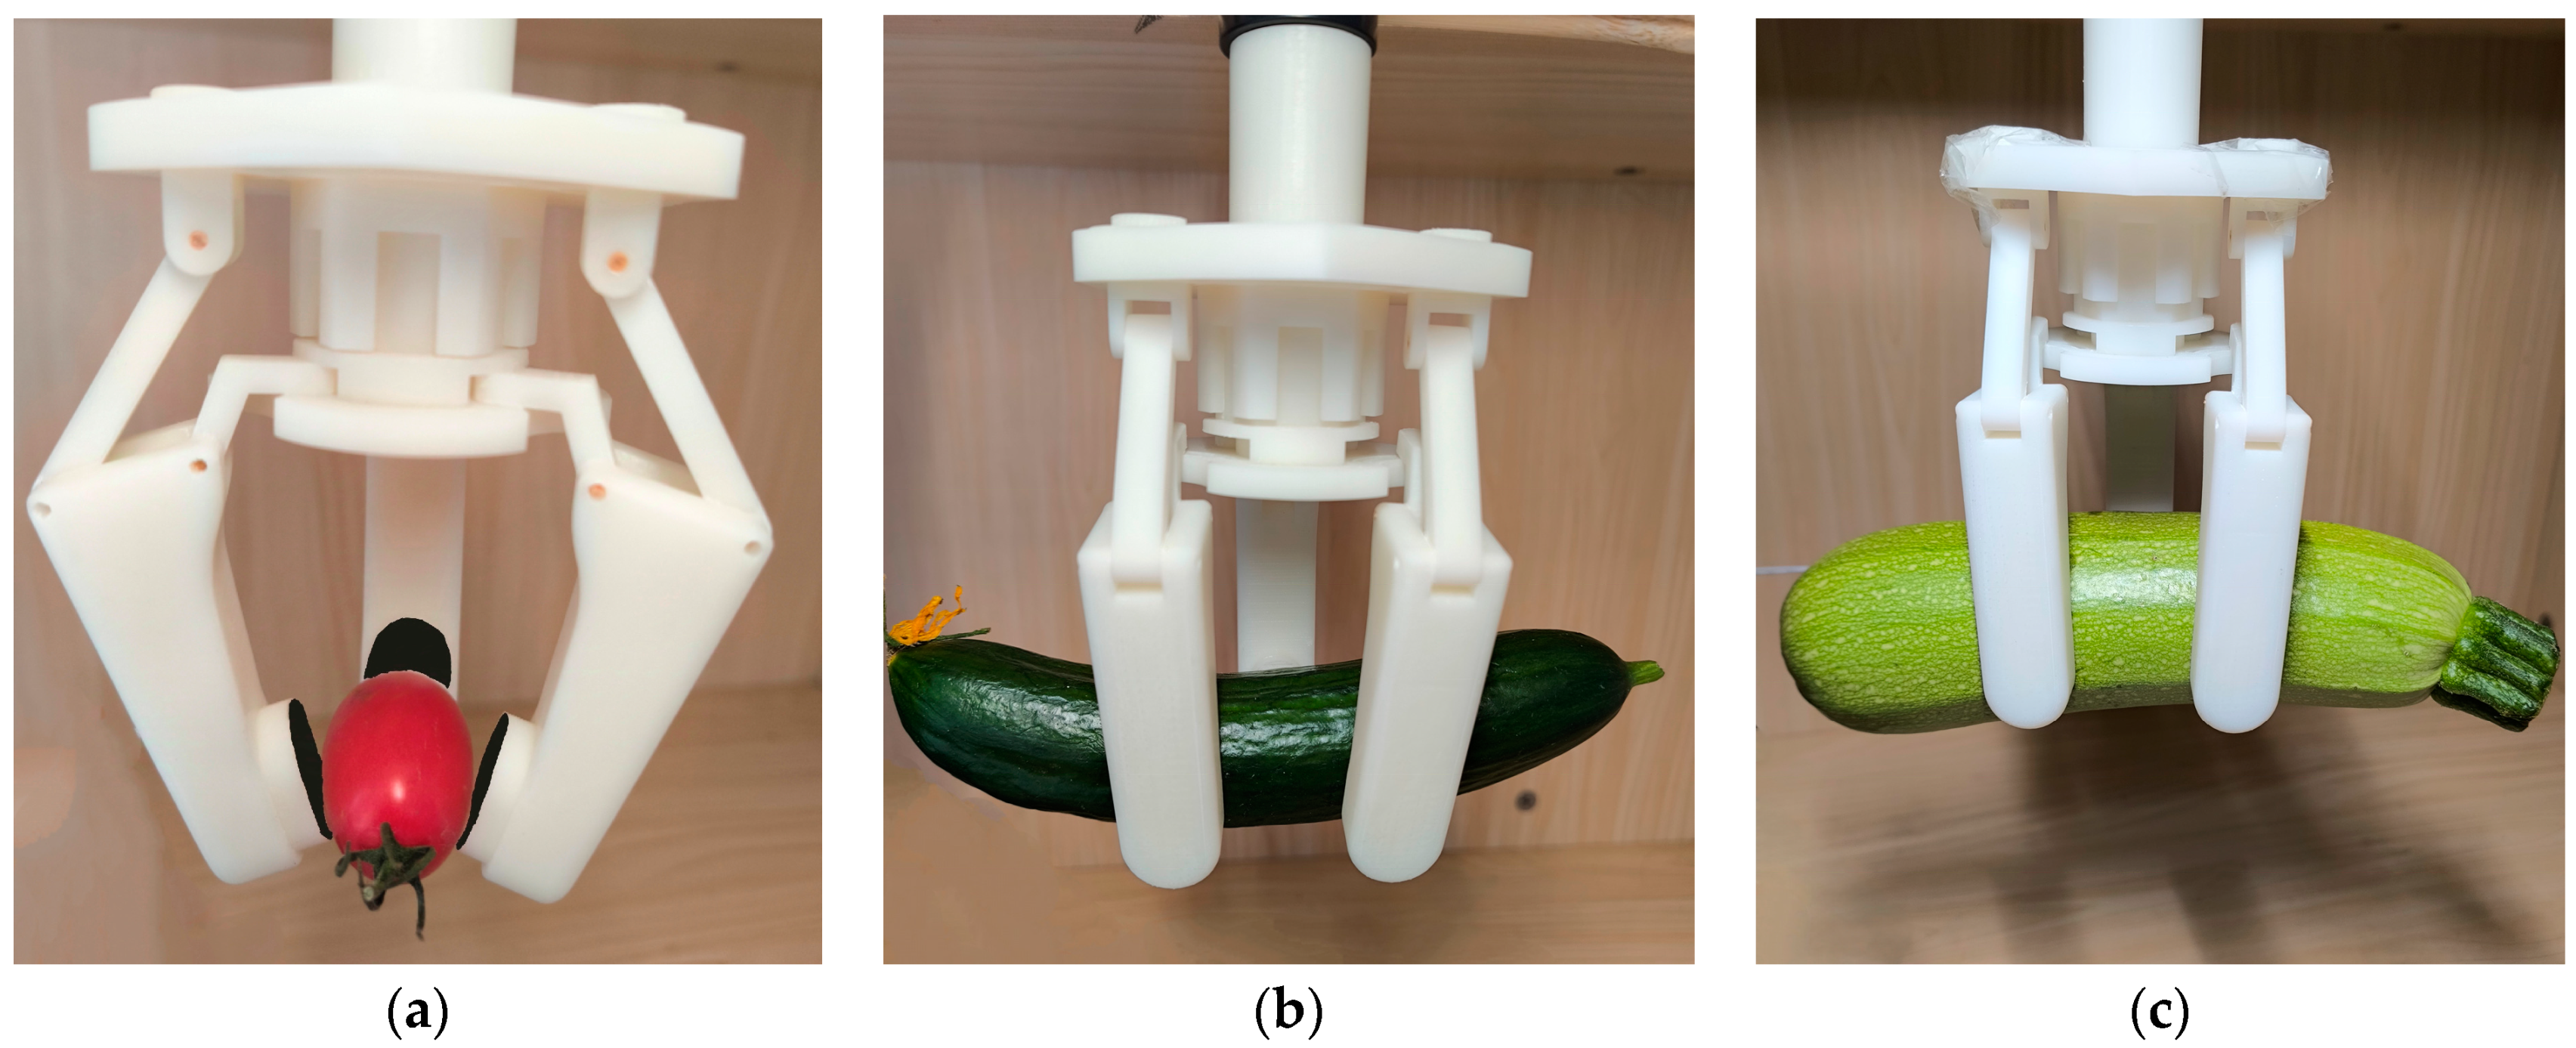
\includegraphics[width=1\linewidth]{pictures/gripper_different_shape.png}
    \caption{Grasping states of different long column strip objects: (a) cherry, (b) loquat, and (c) zucchini.[\cite{multipurpuse_gripper}]}
    \label{fig:enter-label}
\end{figure}

Based on these study, I can conclude that the design for the asparagus gripper should requires a more sophisticated gripper design compared to other fruits/vegetables:

\textbullet \,\textbf{ Unique Morphology}:
Unique Morphology: Asparagus spears have a long, slender, and tapered shape with delicate tips, demanding precise force distribution along their length to avoid bending or snapping, unlike spherical fruits where grip forces can be evenly distributed.\\
\textbullet \,\textbf{ Fragility and Surface Sensitivity:}
Fragility and Surface Sensitivity: The tender skin and high moisture content of asparagus make it prone to bruising or peeling under excessive pressure, necessitating compliant materials and real-time force feedback to adjust grip dynamically.\\
\textbullet \,\textbf{Harvesting Complexity :}
 Asparagus grows at varying angles and densities in the field, requiring grippers with advanced spatial awareness (e.g., 3D vision) and adaptability to selectively harvest mature spears without disturbing adjacent plants.


\section{Comprehensive Analysis: Rationale for \newline Robotics in Asparagus Farming}

Asparagus sprouts, commonly referred to as spears, are harvested primarily by hand in most parts of the world, a method rooted in the crop’s delicate nature and the need for selective picking. Asparagus (Asparagus officinalis) is a perennial plant, with spears emerging from underground crowns in spring and early summer. Harvesting occurs daily or every few days during the 6- to 8-week season, depending on climate and growth rates, as spears must be collected when they reach an optimal height (typically 5-9 inches) before they "fern out" and become fibrous. Workers use knives or snap the spears by hand just above or below the soil surface, depending on market preferences—snapping yields an all-edible product, while cutting below ground adds weight but includes a tougher base often discarded.


In major producing regions like the United States (Michigan, California), Peru, and China, manual labor dominates due to the precision required to assess spear quality and maturity. For instance, in the U.S., where annual production hovers around 20,000-25,000 acres, small-scale farms (often under one acre) rely on seasonal workers or family labor. Larger operations may employ migrant workers, particularly in labor-intensive periods. In contrast, countries like Peru, a leading exporter, benefit from lower labor costs, enabling them to dominate global markets with hand-harvested asparagus. The process involves workers bending or kneeling in fields, collecting spears into buckets or crates, which are then transported for washing, sorting, and packing—often still by hand for premium fresh markets.


Economic and Social Effects
Economically, manual asparagus harvesting has significant implications. It’s labor-intensive, with labor costs constituting a large portion of production expenses—sometimes up to 50 or more, depending on wages and region. In the U.S., where farmgate value ranges from 70-100 million annually, growers face competition from imports (e.g., Peru and Mexico supply 80-90 of U.S. consumption), which depresses domestic prices and squeezes margins. Small-scale farmers benefit from niche markets like farmers' markets or CSAs, fetching premium prices (3-5 per pound), but larger producers struggle with scale and cost efficiency. Rising labor costs, driven by minimum wage increases or labor shortages, further challenge profitability, especially as U.S. acreage has declined to a third of its level two decades ago due to import pressure.
Socially, the reliance on manual labor ties asparagus production to broader workforce dynamics. In developed nations, it sustains seasonal employment, often for migrant or rural communities, providing income but also perpetuating low-wage, physically demanding jobs. In the U.S., for example, many workers are immigrants, highlighting issues of labor rights, housing, and access to services. In developing countries like Peru, asparagus harvesting supports rural livelihoods but can reinforce economic disparities, as smallholders may lack bargaining power against exporters. Gender roles also emerge—women often participate in sorting and packing, while men dominate field work—reflecting traditional divisions with varying social equity implications. Additionally, 

\begin{figure}
    \centering
    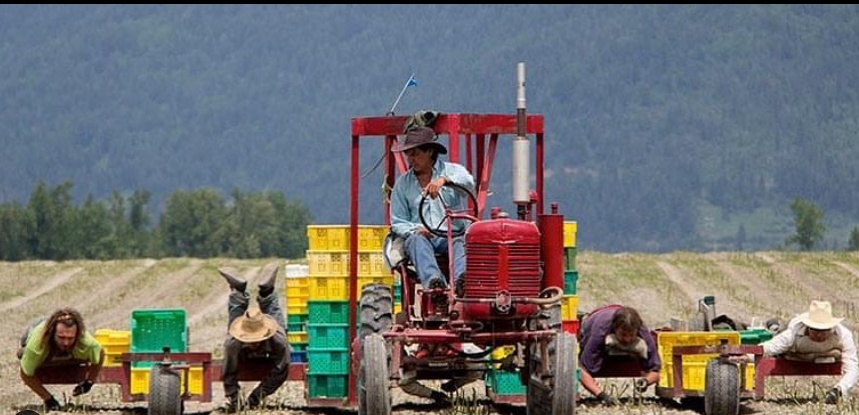
\includegraphics[width=1\linewidth]{pictures/picking_labour.png}
    \caption{manual process of picking spear from field}
    \label{fig:enter-label}
\end{figure}
	

labor shortages, exacerbated by aging rural populations and urban migration (e.g., China’s rural workforce over 60 exceeds 23 per recent census trends), strain production capacity, prompting a push for [\cite{mccluskey2007economics}] and agricultural mechanization trends alternatives which is outlined in the following table \ref{tab:benefits}





\begin{table}[h]
    \centering
    \renewcommand{\arraystretch}{1.3}
    \begin{tabular}{|l|p{6cm}|p{5cm}|}
        \hline
        \textbf{Aspect} & \textbf{Importance} & \textbf{Quantifiable Benefit} \\
        \hline
        \textbf{Cost Reduction} & Lowers labor dependency, stabilizing expenses. & 30-50 percent reduction in harvest costs. \\
        \hline
        \textbf{Yield Consistency} & Ensures timely picking, reducing spoilage. & 10-15 percent increase in marketable yield. \\
        \hline
        \textbf{Scalability} & Enables large-scale operations to compete globally. & 2-3x acreage capacity/farm. \\
        \hline
        \textbf{Sustainability} & Reduces resource waste and supports precision harvesting. & 5-10 percent less water/fertilizer use. \\
        \hline
        \textbf{Labor Relief} & Frees workers for higher-value tasks, improving rural economies. & 20-30 percent labor reallocation potential. \\
        \hline
    \end{tabular}
    \caption{Table showing the importance and benefits of various aspects.}
    \label{tab:benefits}
\end{table}




\subsection{Selective Robotic Harvesters with Vision Systems}
Among the most promising advancements in asparagus harvesting automation are selective robotic harvesters equipped with vision systems, a technology that has gained traction in recent years as labor costs soar and workforce availability dwindles. These systems, such as the ``Sprout'' harvester developed by Muddy Machines in the UK and the SPARTerS [\cite{cordis2025}] project’s underground detection robot in Europe, rely on sophisticated imaging—ranging from RGB cameras to stereo vision and Time-of-Flight sensors—to identify asparagus spears ready for harvest. The process begins with the system scanning the field, detecting spears based on height, thickness, and maturity, then directing a robotic arm to either cut or grasp them with precision. The ``Sprout'' machine, trialed in 2022 with Britain’s largest asparagus grower[\cite{muddymachines2025}], boasts an impressive capacity of 15 acres per day, roughly equivalent to a small human crew, while the SPARTerS robot, designed for white asparagus, uses subsurface sensors to locate spears beneath soil mounds, avoiding damage to the delicate crowns that ensure future yields. These innovations have found footing in high-labor-cost regions like the UK, Netherlands, Germany, and New Zealand, where growers face wages exceeding \$15--20 per hour and seasonal labor shortages driven by urban migration and aging rural populations. The appeal lies in their ability to mimic human selectivity, a critical requirement for fresh asparagus markets where uniformity and tenderness command premium prices—often \$3--5 per pound in local U.S. markets or €4--6 per kilogram in Europe.

The development of these systems reflects a broader push toward precision agriculture, spurred by advancements in AI and robotics over the past decade. Early prototypes, emerging around 2015, struggled with basic image recognition, but by 2020, projects like SPARTerS—funded through EU Horizon programs[\cite{pnoconsultants_horizon}]—integrated machine learning to boost accuracy. Today, they’re piloted on farms covering hundreds of acres, with companies touting labor cost reductions of 30--40\% over manual methods. Yet, their adoption remains limited, concentrated among large-scale producers who can absorb the steep initial investment—units like the ``Sprout'' harvester retail for upwards of \$450,000, plus maintenance costs that can add \$50,000 annually[\cite{muddymachines2025}][\cite{muddymachines2025}]. For smaller farms, which dominate U.S. asparagus production (75\% under one acre per Penn State Extension, 2021), this price tag is prohibitive, locking them into traditional labor models despite competitive pressures from imports like Peru, which supplies 60\% of U.S. consumption at lower costs.

Another important innovation from the east where they utilized 3 DOF robot arm with spring loaded mechanism to make the whole operation light weight and agile as possible as shown in the figure . The Mainichi Japan article from December 15, 2019, reports that Japan’s Ministry of Agriculture, Forestry and Fisheries (MAFF) is investing 100 million yen to develop an asparagus harvesting robot, aiming to address labor shortages in the country’s 5,000-hectare asparagus industry. The robot, designed to pick 1,000 spears per hour, targets export markets like Europe and North America, where labor costs are high. It features a mobile platform with vision-guided robotic arms, as shown in an accompanying image of the system harvesting green asparagus.According to report,  Given its design for a controlled 1,000 spears/hour pace, it likely struggles with real-world variability, lacking the adaptability your 3D stereo camera and point cloud data could provide for better spatial mapping and navigation[\cite{mainichi2019asparagus}].



\begin{figure}
    \centering
    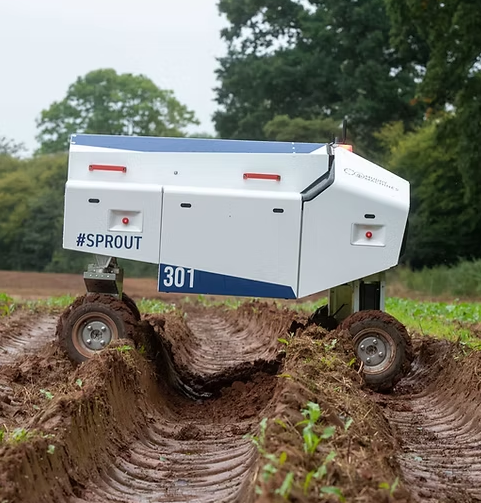
\includegraphics[width=0.75\linewidth]{pictures/muddyMachine.png}
    \caption{sprout from muddy machine}
    \label{fig:enter-label}
\end{figure}
	

\begin{figure}
    \centering
    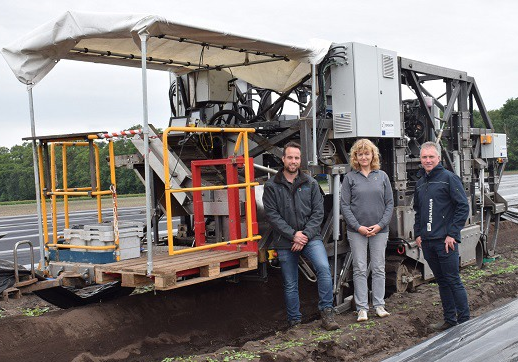
\includegraphics[width=0.75\linewidth]{pictures/spingel.png}
    \caption{SPARTerS project from GERMANY}
    \label{fig:enter-label}
\end{figure}

\begin{figure}
    \centering
    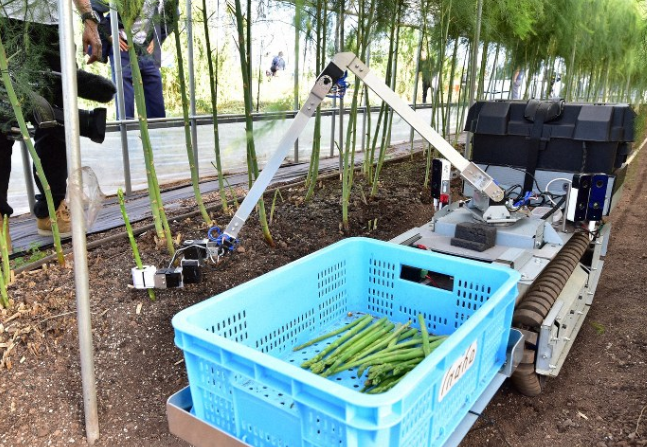
\includegraphics[width=0.75\linewidth]{pictures/INAHOROBOT.png}
    \caption{robot from inaho working in greenhouse environment}
    \label{fig:enter-label}
\end{figure}



The limitations of these robotic harvesters are as significant as their potential. Field tests reveal inconsistent performance in real-world conditions—success rates drop from 90\% in controlled settings to 77\% in cluttered fields where spears grow less than 10 cm apart, as noted in \textit{Mobile Robot System for Selective Asparagus Harvesting} [\cite{mdpi2023mobile}]. Uneven terrain, muddy patches, or low-light conditions further erode reliability, with studies like \textit{Robotic Harvesting of Asparagus using Machine Learning and Time-of-Flight Imaging} [\cite{peebles2022robotic}] reporting a 92.3\% detection rate that plummets after dusk. Economically, their high cost yields a slow return on investment, requiring years of operation across a short 6--8 week season to break even, a challenge compounded by the need for trained technicians in rural areas[\cite{waea2004simulation}]. Socially, they risk displacing seasonal workers, a concern in regions like Michigan or Spain where asparagus harvesting supports migrant and rural livelihoods. What these systems lack is affordability to democratize access, robust adaptability to diverse environmental variables, and the nuanced decision-making humans employ when faced with partially hidden spears or unexpected obstacles—gaps.

\subsection{Nonselective Mechanical Harvesters}
A more established, though less versatile, automation method is the nonselective mechanical harvester, which has been used for decades in asparagus production, particularly for processed markets like canning or freezing. Unlike selective robots, these machines operate on a simpler principle: a blade or cutting bar, mounted on a tractor or mobile frame, sweeps through the field at a fixed height—typically 1--2 inches above or below the soil—harvesting all spears in its path regardless of size or maturity. After collection, workers or secondary machines sort the haul, separating marketable spears from those too small or over-mature. This approach is most common in industrial-scale operations, such as those in China (the world’s top producer at over 7 million tons annually) or the U.S., where companies like Seneca Foods use it for processed asparagus sold at \$1--2 per can. Its roots trace back to the 1970s, when rising labor costs first prompted mechanization experiments, though early designs were crude and wasteful, cutting more than they salvaged[\cite{usda2022labor}].

Globally, nonselective harvesters persist in niche roles because of their lower cost—ranging from \$50,000 to \$150,000—and straightforward maintenance, appealing to producers prioritizing volume over quality[\cite{usda2023asparagus}]. In regions like Peru, which exports 120,000 tons yearly, they complement manual labor for secondary harvests, capturing spears missed by workers. However, their economic viability is narrow. Simulations from \textit{Simulation of Harvesting Asparagus: Mechanical vs. Manual} [\cite{waea2004simulation}] show a recovery rate of just 50--60\% compared to manual harvesting, well below the 72--73\% threshold needed to match human profitability for fresh markets. This inefficiency stems from cutting unripe spears, which stunts future growth, and damaging crowns, reducing yields in subsequent seasons by up to 10--15\%. For fresh asparagus, where consumers demand spears of consistent length and tenderness, the method falls flat, relegating it to processed goods where quality standards are laxer[\cite{usda2023asparagus}].

The limitations are stark: nonselective harvesters lack the selectivity to preserve unharvested spears or meet fresh market demands, a critical flaw as fresh asparagus accounts for 70\% of U.S. retail value [\cite{usda2023asparagus}]. They also pose sustainability risks—overharvesting weakens plant longevity, clashing with modern goals of resource efficiency. Socially, they reduce labor needs but don’t eliminate them entirely, as sorting remains manual, perpetuating low-wage jobs without addressing broader workforce shortages. What’s missing is the ability to adapt to selective harvesting needs, minimize long-term crop damage, and integrate with systems that prioritize quality over sheer volume—an area where your proposed technology could offer a smarter alternative.

\subsection{Harvest Assist Technologies}
Harvest assist technologies offer a pragmatic bridge between manual and fully automated harvesting, supporting workers rather than replacing them. Machines like the ``asparagus spider'' from Engels Machines in the Netherlands or mobile conveyor platforms are designed to ease the physical burden of picking asparagus. The ``spider,'' widely used for white asparagus in Europe, manages the plastic foil that keeps spears blanched, while workers cut and place them onto a conveyor that ferries them to crates, doubling hourly output from 10--15 kg to 20--30 kg per worker[\cite{freshplaza2019automation}]. Similar platforms for green asparagus, seen in California or New Zealand, allow pickers to work upright, reducing fatigue from bending across 20-acre fields. These tools have gained traction since the early 2000s, with adoption rates reaching 20--30\% in European asparagus regions and growing elsewhere as labor costs climb—e.g., €12--15/hour in Germany versus \$1--2/hour in Peru[\cite{freshplaza2018engels}][\cite{engelsmachines2020about}].

Their appeal lies in affordability and simplicity—costing \$20,000--\$50,000, they’re within reach for mid-sized farms, offering a 5--10\% reduction in labor expenses without the upheaval of full automation. In practice, they’ve transformed workflows, especially for white asparagus, where foil management once consumed hours daily. Reports like \textit{“Higher level of automation leads to better asparagus product quality”} [\cite{freshplaza2019automation}] praise their role in boosting consistency, as rested workers make fewer errors. Yet, They still depend on human labor, leaving growers exposed to shortages—U.S. farms lost 10--15\% of their workforce to urban jobs in the past decade [\cite{usda2022labor}]. Their economic impact is modest, shaving costs but not enough to compete with low-wage imports, and they don’t scale well for vast operations needing dozens of workers.

What these technologies lack is the leap to full automation, leaving the core challenge of labor dependency unresolved. They also miss advanced decision-making to optimize picking beyond human input, and their integration with broader production systems—planting, sorting, packing—remains rudimentary. Socially, they improve worker conditions but don’t address job precarity, as seasonal roles persist. Your thesis’s LLM-driven robotic arm could push beyond this assist model, offering a fully autonomous solution that these tools only hint at.

An emerging frontier in asparagus automation involves delta robot systems mounted on mobile platforms, a concept gaining attention through research like \textit{Mobile Robot System for Selective Asparagus Harvesting} [\cite{mdpi2023mobile}]. These systems feature lightweight, tripod-like delta arms—known for their speed in industrial settings—mounted on tracked or wheeled bases that roam open fields. Guided by real-time vision algorithms, they detect green asparagus spears and pick them in roughly 3.5 seconds per cycle, a pace that rivals human workers in controlled conditions. Developed through lab and field trials, primarily in Germany, they’ve achieved an 88\% success rate in test plots, targeting small- to mid-sized farms where flexibility matters. Their design evolved from factory robotics, adapted since 2018 for agriculture’s rougher terrain, with prototypes now navigating rows up to 500 meters long[\cite{sparters2020automated}].
\begin{figure}
    \centering
    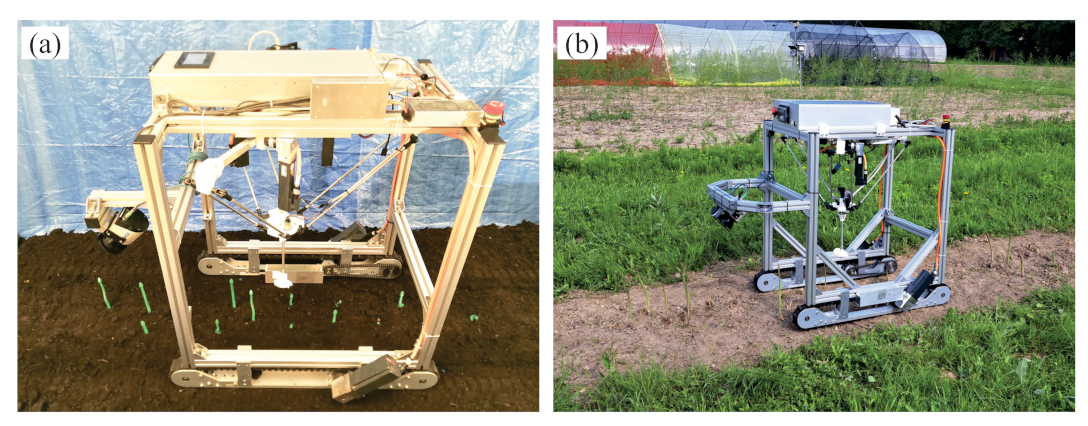
\includegraphics[width=0.75\linewidth]{pictures/delta_robot.png}
    \caption{Delta Robot Systems on Mobile Platform}
    \label{fig:enter-label}
\end{figure}





Their potential is compelling: delta robots are faster than traditional robotic arms, and their mobility suits the scattered layouts of asparagus fields. In Germany, where labor costs hit €15/hour, they promise a 20--30\% reduction in harvest expenses if scaled commercially. However, field performance lags—success drops to 77\% when spears grow too close or terrain shifts, as mislocalized picking points lead to misses. The MDPI study notes energy constraints, with batteries lasting 6--8 hours, insufficient for 24-hour harvest windows in peak season. Costs, while lower than selective harvesters (estimated \$200,000--\$300,000), remain a barrier, and their experimental status limits adoption to research-backed farms rather than widespread use[\cite{mdpi2023mobile}].

These systems lack the precision and speed to fully replace humans in uncontrolled settings, as well as the energy efficiency for extended operation. They also struggle with commercialization—high R\&D costs slow mass production, and small farms can’t justify the investment[\cite{waea2004simulation}].


\section{Open Challenges}



Developing an AI-driven robotic arm for asparagus harvesting, powered by large language models (LLMs) and computer vision, presents significant challenges that must be navigated to achieve success. The first major hurdle is the high development cost. Creating a prototype requires expensive hardware—high-resolution cameras, precise actuators, and robust robotic arms\newline combined with extensive software development to train computer vision models and LLMs on asparagus-specific datasets.Cloud or edge computing resources for LLMs further inflate expenses, potentially limiting accessibility without subsidies or partnerships. Another challenge is the complexity of field conditions. Asparagus grows in uneven terrain with variable lighting, shadows, and weed occlusion, which can reduce computer vision accuracy below 90 percent in adverse conditions like rain or dusk.


My motivation to improve the field of asparagus farming through an AI-driven robotic arm, powered by large language models (LLMs) and computer vision, stems from a deep desire to address pressing challenges and transform agricultural practices for a sustainable future. Asparagus harvesting is labor-intensive, requiring workers to painstakingly cut spears at precise moments to ensure quality and crown health, yet farms worldwide face acute labor shortages, with seasonal worker availability dropping by 20 percent in regions like North America since 2020 . By developing a robotic arm that autonomously identifies and picks asparagus using computer vision, I aim to alleviate this burden, enabling farms to maintain output without relying on scarce human labor. Systems like Octinion’s asparagus robot inspire this vision, demonstrating that vision-based automation can match human precision . Beyond labor, I am driven to enhance harvest precision. Asparagus quality depends on cutting spears at the right length and maturity, a task where errors reduce market value by up to 15 percent. Computer vision, trained on diverse field datasets, can achieve over 95 percent accuracy in spear detection. This precision not only boosts farm revenue but also strengthens food security as global asparagus demand grows by 4 percent annually. Efficiency is another core motivator. Manual harvesting is slow, with workers averaging 3-5 seconds per spear, limiting scalability as labor costs consume half of production budgets. My goal is a robotic arm that picks in under a second, operating 24/7 to maximize yield and minimize waste, allowing farms to scale without proportional cost increases. LLMs could coordinate multiple arms, streamlining large-scale operations. Sustainability further fuels my passion.

